%!TEX TS-program = xelatex
\documentclass[12pt, a4paper, oneside]{article}

% Можно вставить разную преамбулу
\input{preamble}

% для нормального распределения
\newcommand{\expp}[1]{ \exp \left( #1 \right)} 
% для прорисовки нормального распределения
\newcommand\gauss[2]{1/(#2*sqrt(2*pi))*exp(-((x-#1)^2)/(2*#2^2))} 


\title{\begin{center} \includegraphics[width=0.99\textwidth]{logo.png} \end{center} К чёрту условности!\footnote{Эта pdf-ка, по факту, представляет из себя кусочек недописанной виньетки по Байесовским методам: \newline  \url{https://github.com/FUlyankin/book_about_bayes}}}
% \author{Ульянкин Филя, Романенко Саша}

\begin{document}
	
	\maketitle
	
\epigraph{Ты здоров на 91\%, когда все вокруг говорят, что ты болен на 99\%}{}


\section{Условные вероятности}


Поговорим о гороскопах. У тёти Маши --- двое детей разных возрастов. Вероятности рождения мальчика и девочки равны.

\begin{enumerate}
\item Какова вероятность того, что у тёти Маши оба ребёнка --- мальчики, если известно, что у неё хотя бы один ребёнок -- мальчик?
\item Какова вероятность того, что у тёти Маши оба ребёнка --- мальчики, если известно, что у неё хотя бы один ребёнок --- мальчик да ещё и стрелец по гороскопу?
\end{enumerate}


Давайте вспомним семинары по терверу. Скорее всего, для таких задачек, читатель обычно рисовал дерево. Не будем далеко ходить и сделаем то же самое.

\begin{center}
\definecolor{qqqqff}{rgb}{0.,0.,1.}
\begin{tikzpicture}[line cap=round,x=1.0cm,y=1.0cm]
\clip(-0.39363012181616935,-2.006361018826134) rectangle (8.805926910299,3.314569213732001);
\draw [->] (-0.06,0.46) -- (1.9647308970099653,1.560416389811739);
\draw [->] (-0.06,0.46) -- (1.945240310077518,0.8197740863787383);
\draw [->] (-0.06,0.46) -- (1.9647308970099653,0.21556589147286925);
\draw [->] (-0.06,0.46) -- (2.0621838316722023,-0.6030387596899212);
\draw (3.161904761904762,1.9610188261351054)-- (3.161904761904762,-1.0389811738648946);
\draw (4.8,1.9610188261351051)-- (4.8,-1.0389811738648949);
\draw (8.201718715393131,1.9621882613510533)-- (8.201718715393131,-1.0378117386489467);
\draw (2.2,1.9) node[anchor=north west] {$\text{ММ}$};
\draw (2.2,1.1) node[anchor=north west] {$\text{МД}$};
\draw (2.2,0.5) node[anchor=north west] {$\text{ДМ}$};
\draw (2.2,-0.3) node[anchor=north west] {$\text{ДД}$};
\draw (3.4,1.9) node[anchor=north west] {$0.25$};
\draw (3.4,1.1) node[anchor=north west] {$0.25$};
\draw (3.4,0.5) node[anchor=north west] {$0.25$};
\draw (3.4,-0.3) node[anchor=north west] {$0.25$};
%\draw (3.1,2.55) node[anchor=north west] {$\text{Не знаю}$};
\draw (5,2.55) node[anchor=north west] {\parbox{3.8066445182724244 cm}{$\text{Хотя бы один М}$}};
\draw (6.1,1.9) node[anchor=north west] {$^1/_3$};
\draw (6.1,1.1) node[anchor=north west] {$^1/_3$};
\draw (6.1,0.5) node[anchor=north west] {$^1/_3$};
\draw (6.2,-0.3) node[anchor=north west] {$0$};
\begin{scriptsize}
\draw [fill=qqqqff] (-0.06,0.46) circle (2.5pt);
\end{scriptsize}
\end{tikzpicture}
\end{center}

До~поступления информации о том, что в~семье имеется один мальчик, вероятности получить каждую пару детей были одинаковыми. После того, как стало известно, что хотя бы один ребёнок является мальчиком, вероятность исхода ДД занулилась. Остальные вероятности, в~связи~с поступлением новой информации, должны как-то поменяться, чтобы в сумме давать единицу. Поскольку, как мальчик, так и девочка в~качестве второго ребёнка равновероятны, то они возрастают пропорционально до~$\frac{1}{3}$. Условие, словно садовник, срезает одну из ветвей дерева. 

Можно посчитать всё это по-честному. Вспомним формулу условной вероятности
\[ \PP(\text{MM} \mid \text{Хотя бы один М}) = \frac{\PP(\text{MM}, \text{Хотя бы один М})}{  \PP(\text{Хотя бы один М})} = \frac{0.25}{1 - 0.25} = \frac{1}{3}.\]

Хорошо. Теперь найдём вероятность того, что у тёти Маши два мальчика при условии, что один из них стрелец. Для этого снова нарисуем дерево.

\begin{center}
\definecolor{qqqqff}{rgb}{0.,0.,1.}
\begin{tikzpicture}[scale=0.9, line cap=round,x=1.0cm,y=1.0cm]
\clip(-3.76,-1.3) rectangle (10.34,5.64);
\draw [->] (2.,5.) -- (0.,3.);
\draw [->] (2.,5.) -- (4.,3.);
\draw [->] (0.,3.) -- (-2.,2.);
\draw [->] (0.,3.) -- (1.,2.);
\draw [->, dash pattern=on 5pt off 5pt] (-2.,2.) -- (-3.,0.);
\draw [->, dash pattern=on 5pt off 5pt] (-2.,2.) -- (-1.,0.);
\draw [->, dash pattern=on 5pt off 5pt] (4.,3.) -- (3.,2.);
\draw [->, dash pattern=on 5pt off 5pt] (4.,3.) -- (6.,2.);
\draw [->] (6.,2.) -- (8.,3.);
\draw [->] (6.,2.) -- (7.,1.);
\draw [->, dash pattern=on 5pt off 5pt] (7.,1.) -- (9.,1.);
\draw [->, dash pattern=on 5pt off 5pt] (7.,1.) -- (8.,0.);
\draw [->] (3.,2.) -- (2.,1.);
\draw [->] (3.,2.) -- (4.,1.);
\draw [->, dash pattern=on 5pt off 5pt] (4.,1.) -- (3.,0.);
\draw [->, dash pattern=on 5pt off 5pt] (4.,1.) -- (5.,0.);
\draw (-0.36,4.18) node[anchor=north west] {$\text{Д}$};
\draw (4.06,4.18) node[anchor=north west] {$\text{М}$};
\draw (0.98,2.98) node[anchor=north west] {$\text{Д}$};
\draw (-2.58,2.9) node[anchor=north west] {$\text{М}$};
\draw (-3.46,-0.1) node[anchor=north west] {$\text{МС}$};
\draw (-1.5,0.02) node[anchor=north west] {$\text{не МС}$};
\draw (8.24,3.84) node[anchor=north west] {$\text{Д}$};
\draw (1.32,1.34) node[anchor=north west] {$\text{Д}$};
\draw (4.28,1.56) node[anchor=north west] {$\text{М}$};
\draw (6.9,2.) node[anchor=north west] {$\text{М}$};
\draw (2.64,-0.06) node[anchor=north west] {$\text{МС}$};
\draw (9.16,1.8) node[anchor=north west] {$\text{МС}$};
\draw (3.28,2.52) node[anchor=north west] {$\text{не МС}$};
\draw (5.62,3.16) node[anchor=north west] {$\text{МС}$};
\draw (4.72,-0.04) node[anchor=north west] {$\text{не МС}$};
\draw (7.8,0.04) node[anchor=north west] {$\text{не МС}$};
\begin{scriptsize}
\draw [fill=qqqqff] (2.,5.) circle (2.5pt);
\draw [fill=qqqqff] (0.,3.) circle (2.5pt);
\draw [fill=qqqqff] (4.,3.) circle (2.5pt);
\draw [fill=qqqqff] (-2.,2.) circle (2.5pt);
\draw [fill=qqqqff] (1.,2.) circle (2.5pt);
\draw [fill=qqqqff] (-3.,0.) circle (2.5pt);
\draw [fill=qqqqff] (-1.,0.) circle (2.5pt);
\draw [fill=qqqqff] (3.,2.) circle (2.5pt);
\draw [fill=qqqqff] (6.,2.) circle (2.5pt);
\draw [fill=qqqqff] (8.,3.) circle (2.5pt);
\draw [fill=qqqqff] (7.,1.) circle (2.5pt);
\draw [fill=qqqqff] (9.,1.) circle (2.5pt);
\draw [fill=qqqqff] (8.,0.) circle (2.5pt);
\draw [fill=qqqqff] (2.,1.) circle (2.5pt);
\draw [fill=qqqqff] (4.,1.) circle (2.5pt);
\draw [fill=qqqqff] (3.,0.) circle (2.5pt);
\draw [fill=qqqqff] (5.,0.) circle (2.5pt);
\end{scriptsize}
\end{tikzpicture}
\end{center}

Новое дерево получилось развесистым. Развесистости добавляют пунктирные ветки, отвечающие за гороскоп. По ветке $\text{МС}$ мы проходим с вероятностью $\frac{1}{12}$. По обычным, не пунктирным, веткам мы проходим с вероятностью $\frac{1}{2}$. У тёти Маши есть один мальчик, и он стрелец. Это означает, что мы хотя бы разочек должны пройти по пунктирной ветке с надписью $\text{МС}$.  Это ограничение состригает c дерева некоторые ветки и даёт нам пять траекторий.

\begin{center}
\definecolor{ffffqq}{rgb}{1.,1.,0.}
\definecolor{ffqqqq}{rgb}{1.,0.,0.}
\definecolor{qqqqff}{rgb}{0.,0.,1.}
\begin{tikzpicture}[scale=0.9,x=1.0cm,y=1.0cm]
\clip(-3.76,-1.3) rectangle (10.34,5.64);
\draw [->] (2.,5.) -- (0.,3.);
\draw [->] (2.,5.) -- (4.,3.);
\draw [->] (0.,3.) -- (-2.,2.);
\draw [->] (0.,3.) -- (1.,2.);
\draw [->,dash pattern=on 5pt off 5pt] (-2.,2.) -- (-3.,0.);
\draw [->, dash pattern=on 5pt off 5pt] (-2.,2.) -- (-1.,0.);
\draw [->,dash pattern=on 5pt off 5pt] (4.,3.) -- (3.,2.);
\draw [->,dash pattern=on 5pt off 5pt] (4.,3.) -- (6.,2.);
\draw [->] (6.,2.) -- (8.,3.);
\draw [->] (6.,2.) -- (7.,1.);
\draw [->,dash pattern=on 5pt off 5pt] (7.,1.) -- (9.,1.);
\draw [->,dash pattern=on 5pt off 5pt] (7.,1.) -- (8.,0.);
\draw [->] (3.,2.) -- (2.,1.);
\draw [->] (3.,2.) -- (4.,1.);
\draw [->,dash pattern=on 5pt off 5pt] (4.,1.) -- (3.,0.);
\draw [->,dash pattern=on 5pt off 5pt] (4.,1.) -- (5.,0.);
\draw (-0.36,4.18) node[anchor=north west] {$\text{Д}$};
\draw (4.06,4.18) node[anchor=north west] {$\text{М}$};
\draw (0.98,2.98) node[anchor=north west] {$\text{Д}$};
\draw (-2.58,2.9) node[anchor=north west] {$\text{М}$};
\draw (-3.46,-0.1) node[anchor=north west] {$\text{МС}$};
\draw (-1.5,0.02) node[anchor=north west] {$\text{не МС}$};
\draw (8.24,3.84) node[anchor=north west] {$\text{Д}$};
\draw (1.32,1.34) node[anchor=north west] {$\text{Д}$};
\draw (4.28,1.56) node[anchor=north west] {$\text{М}$};
\draw (6.9,2.) node[anchor=north west] {$\text{М}$};
\draw (2.64,-0.06) node[anchor=north west] {$\text{МС}$};
\draw (9.16,1.8) node[anchor=north west] {$\text{МС}$};
\draw (3.28,2.52) node[anchor=north west] {$\text{не МС}$};
\draw (5.62,3.16) node[anchor=north west] {$\text{МС}$};
\draw (4.72,-0.04) node[anchor=north west] {$\text{не МС}$};
\draw (7.8,0.04) node[anchor=north west] {$\text{не МС}$};
\draw [line width=2.8pt,color=ffqqqq] (2.,5.)-- (0.,3.);
\draw [line width=4.4pt,color=ffffqq] (2.,5.)-- (0.,3.);
\draw [line width=4.4pt,color=ffffqq] (0.,3.)-- (-2.,2.);
\draw [line width=4.4pt,color=ffffqq] (-2.,2.)-- (-3.,0.);
\draw [line width=4.4pt,color=ffffqq] (2.,5.)-- (4.,3.);
\draw [line width=4.4pt,color=ffffqq] (4.,3.)-- (6.,2.);
\draw [line width=4.4pt,color=ffffqq] (6.,2.)-- (8.,3.);
\draw [line width=4.4pt,color=ffffqq] (6.,2.)-- (7.,1.);
\draw [line width=4.4pt,color=ffffqq] (7.,1.)-- (9.,1.);
\draw [line width=4.4pt,color=ffffqq] (4.,3.)-- (3.,2.);
\draw [line width=4.4pt,color=ffffqq] (3.,2.)-- (4.,1.);
\draw [line width=4.4pt,color=ffffqq] (4.,1.)-- (3.,0.);
\draw [line width=4.4pt,color=ffffqq] (7.,1.)-- (8.,0.);
\begin{scriptsize}
\draw [fill=qqqqff] (2.,5.) circle (2.5pt);
\draw [fill=qqqqff] (0.,3.) circle (2.5pt);
\draw [fill=qqqqff] (4.,3.) circle (2.5pt);
\draw [fill=qqqqff] (-2.,2.) circle (2.5pt);
\draw [fill=qqqqff] (1.,2.) circle (2.5pt);
\draw [fill=qqqqff] (-3.,0.) circle (2.5pt);
\draw [fill=qqqqff] (-1.,0.) circle (2.5pt);
\draw [fill=qqqqff] (3.,2.) circle (2.5pt);
\draw [fill=qqqqff] (6.,2.) circle (2.5pt);
\draw [fill=qqqqff] (8.,3.) circle (2.5pt);
\draw [fill=qqqqff] (7.,1.) circle (2.5pt);
\draw [fill=qqqqff] (9.,1.) circle (2.5pt);
\draw [fill=qqqqff] (8.,0.) circle (2.5pt);
\draw [fill=qqqqff] (2.,1.) circle (2.5pt);
\draw [fill=qqqqff] (4.,1.) circle (2.5pt);
\draw [fill=qqqqff] (3.,0.) circle (2.5pt);
\draw [fill=qqqqff] (5.,0.) circle (2.5pt);
\end{scriptsize}
\end{tikzpicture}
\end{center}

Просуммируем вероятности пройти по каждой из траекторий и получим вероятность того, что у нас родится хотя бы один мальчик стрелец

\begin{multline*}
\PP( \text{хотя бы один МС}) = 0.5 \cdot 0.5 \cdot \frac{1}{12} + 0.5 \cdot \left( \frac{11}{12} \cdot 0.5 \cdot \frac{1}{12} +  \right. \\ + \frac{1}{12} \cdot \left( 0.5 + 0.5 \cdot \left. \left( \frac{1}{12} + \frac{11}{12} \right) \right) \right) \approx 0.0815.
\end{multline*}

Фактически, мы сейчас использовали формулу полной вероятности, чтобы найти вероятность события <<хотя бы один МС>>, просуммировав его появление при всех возможных гипотезах: $\text{МС и Д}$, $\text{МС и не МС}$, $\text{МС и Д}$, $\text{МС и МС}$, $\text{МС и не МС}$.

Из рассмотренных пяти траекторий только три приводят нас в лист, где пересекаются события хотя бы один МС и $\text{ММ}$. Сумма вероятностей прохода по этим траекториям составит~$0.0399$. Остаётся только применить формулу условной вероятности:

\[ \PP(\text{MM} \mid \text{Хотя бы один МС}) = \frac{\PP(\text{MM}, \text{Хотя бы один МС})}{  \PP(\text{Хотя бы один МС})} = \frac{0.0399}{0.0815} \approx 0.489.\]

В конечном итоге получаем что-то близкое к~$\frac{1}{2}$.  Удивительно, но информация о том, что мальчик, родившийся у тёти Маши --- стрелец, существенно изменяет вероятность того, что родятся два мальчика. Появление на свет стрельца --- это настолько редкое событие, что для его наступления надо нарожать много мальчиков. Событие $\text{ММ}$ происходит гораздо чаще, чем $\text{ММС}$. 

Интуитивно объяснить полученный результат можно, выбросив из рассмотрения событие, при котором рождается два мальчика стрельца. Оно редкое, зачем обращать на него внимание?

\begin{center}
\definecolor{qqwuqq}{rgb}{0.,0.39215686274509803,0.}
\definecolor{ffqqqq}{rgb}{1.,0.,0.}
\begin{tikzpicture}[x=1.0cm,y=1.0cm]
\clip(-3.52,1.88) rectangle (8.5,4.72);
\draw (-3.02,4.5) node[anchor=north west] {$\text{МД}$};
\draw (-1.44,4.5) node[anchor=north west] {$\text{ДМ}$};
\draw (-0.08,4.5) node[anchor=north west] {$\text{ММ}$};
\draw (-3.12,3.5) node[anchor=north west] {$\text{МCД}$};
\draw (-1.52,3.5) node[anchor=north west] {$\text{ДМС}$};
\draw (-0.06,3.5) node[anchor=north west] {$\text{МСМС}$};
\draw (1.8,3.5) node[anchor=north west] {$\text{МС НМС}$};
\draw (3.94,3.5) node[anchor=north west] {$\text{МНС МС}$};
\draw [color=ffqqqq] (0.,3.52)-- (1.2,2.76);
\draw [color=ffqqqq] (0.12,2.78)-- (1.2,3.5);
\draw [color=qqwuqq] (0.,4)-- (0.72,4);
\draw [color=qqwuqq] (1.92,3)-- (3.5,3);
\draw [color=qqwuqq] (4.12,3)-- (5.78,3);
\draw (1.3,4.5) node[anchor=north west] {$\Rightarrow \frac{1}{3}$};
\draw (6.18,3.5) node[anchor=north west] {$\Rightarrow \frac{1}{2}$};
\end{tikzpicture}
\end{center}

После удаления мелкого варианта как раз и получится наша $\frac{1}{2}$. Мораль первого чуда состоит в том, что дополнительная информация стрижет дерево и перераспределяет вероятностную массу между вариантами. Иногда перераспределение выходит очень неожиданным. 

На самом деле, мы с вами только что использовали формулу Байеса.  Давайте чуть более формально вспомним откуда она берётся.  \indef{Совместная вероятность} --- это вероятность одновременного наступления двух событий  $\PP(A,B)$.  События называются \indef{независимыми}, если вероятность совместного наступления событий равна произведению их вероятностей:

\[ \PP(A,B) = \PP(A) \cdot \PP(B).\]

\indef{Условная вероятность} --- это вероятность наступления одного события, если известно, что произошло другое, $\PP(A \mid B)$.  Она определяется как

\[ \PP(A \mid B) = \frac{\PP(A, B)}{\PP(B)}.\]

Внимательно приглядевшись к формуле, можно заметить, что для независимых событий $P(A \mid B) = P(A).$  Если немного переписать условную вероятность, можно получить, что: 

\[ \PP(A, B) = \PP(A \mid B) \cdot \PP(B) = \PP(B \mid A) \cdot \PP(A), \] 

из чего и вытекает формула Байеса:

\[ \PP(B  \mid A) = \frac{\PP(A \mid B) \cdot \PP(B)}{\PP(A)}.\]

Эта формула позволяет переоценивать наши текущие представления о мире (в формуле это $\PP(B)$), используя новую, поступившую к нам информацию (в формуле это $\PP(A \mid B)$), в качестве переоценки получая новое состояние наших представлений, $\PP(B \mid A)$.  

Другой задачкой, которая иллюстрирует идею переоценки наших знаний, является медицинская диагностика. 


\begin{problem}{(Доктор, что со мной?)}
Предположим, что по планете путешествует чрезвычайно смертоносное заболевание. И имя ему ковонавивус. Им заражается один человек из $10 000$.  Медицинская диагностика очень хорошо развита и люди умеют находить это заболевание с высокой точностью, они обнаруживают его в $99\%$ случаев. Когда заболевания у человека нет, вероятность того, что его найдут составляет $1\%$.  Иначе говоря, $1\%$ это вероятность как ошибки первого рода (анализы нашли болезнь, когда её нет), так и ошибки второго рода (анализы не нашли болезнь, когда она есть). 

Случилось страшное! Обследование показало, что человек болен. Какова вероятность того, что болезни у него на самом деле нет? 
\end{problem}

\begin{sol}
Можно попробовать нарисовать дерево и посмотреть как информация о диагнозе состригает лишние ветки, а мы, на этот раз, посчитаем всё по формулам.

Найдём вероятность того, что у человека найдут болезнь. Это может произойти, если он реально болен и если он не болен, но произошла ошибка.  Пусть событие $A$ означает, что болезнь обнаружили, а событие $B$ означает, что человек реально болен.  Тогда событие $B^{c}$ будет означать, что у человека нет болезни\footnote{Обычно символом $B^c$ обозначают событие, которое является дополнением к событию $B$. Для таких событий $\PP(B) + \PP(B^c) = 1$.}. 

\begin{multline*}
\PP(A)  = \PP(A\mid B) \cdot \PP(B) + \PP(A \mid B^{c})  \cdot \PP(B^{c})  = 0.99 \cdot \frac{1}{10000} + 0.01 \cdot \frac{9999}{10000} \approx 0.01.
\end{multline*}

Обратите ещё раз внимание на то, что мы делаем. Мы ищем вероятность того, что человек болен при всех возможных гипотезах. Так как гипотез дискретное число, мы суммируем вероятности, соответствующие им.  В непрерывном случае мы будем поступать похожим образом.  Интегрируя плотность $f(y \mid x)$ по всем возможным значениям, которые принимает случайная величина $X$, мы будем получать плотность $f(y)$. Интеграл это то же самое, что обычная сумма, но для непрерывного случая.

В конечном итоге, используя формулу байеса, мы можем пересчитать вероятность того, что человек реально болен, при условии, что у него нашли болезнь:

\[  \PP(B \mid A) = \frac{ \PP(A \mid B)\cdot \PP(B) }{\PP(A)}  = \frac{0.99 \cdot \frac{1}{10000}}{0.01} \approx 0.01. \]Читатель может попробовать нарисовать дерево и посмотреть как информация о диагнозе состригает лишние ветки, а мы, на этот раз, посчитаем всё по формулам.

Найдём вероятность того, что у человека найдут болезнь. Это может произойти, если он реально болен и если он не болен, но произошла ошибка.  Пусть событие $A$ означает, что болезнь обнаружили, а событие $B$ означает, что человек реально болен.  Тогда событие $B^{c}$ будет означать, что у человека нет болезни\footnote{Обычно символом $B^c$ обозначают событие, которое является дополнением к событию $B$. Для таких событий $\PP(B) + \PP(B^c) = 1$.}. 

\begin{multline*}
\PP(A)  = \PP(A\mid B) \cdot \PP(B) + \PP(A \mid B^{c})  \cdot \PP(B^{c})  = 0.99 \cdot \frac{1}{10000} + 0.01 \cdot \frac{9999}{10000} \approx 0.01.
\end{multline*}

Обратите ещё раз внимание на то, что мы делаем. Мы ищем вероятность того, что человек болен при всех возможных гипотезах. Так как гипотез дискретное число, мы суммируем вероятности, соответствующие им.  В непрерывном случае мы будем поступать похожим образом.  Интегрируя плотность $f(y \mid x)$ по всем возможным значениям, которые принимает случайная величина $X$, мы будем получать плотность $f(y)$. Интеграл это то же самое, что обычная сумма, но для непрерывного случая.

В конечном итоге, используя формулу байеса, мы можем пересчитать вероятность того, что человек реально болен, при условии, что у него нашли болезнь:

\[  \PP(B \mid A) = \frac{ \PP(A \mid B)\cdot \PP(B) }{\PP(A)}  = \frac{0.99 \cdot \frac{1}{10000}}{0.01} \approx 0.01. \]
\end{sol}


Это что же --- воскликнет возмущённый читатель, --- теперь не верить врачам и лечиться средствами традиционной медицины? Нет. Врачам нужно продолжать доверять, но всегда надо иметь в виду, что в случае, если болезнь довольно слабо распространена, точность диагноза должна быть не $99\%$, а гораздо выше.

Задачку про медицину и болезнь можно встретить почти во всех пособиях и лекциях по байсовским методам. Она является неплохим примером обратной задачи теории вероятностей. 

\indef{Прямые задачи} возникают, когда дано описание некоторого вероятностного процесса, и мы должны найти вероятность того или иного события, то есть по модели предсказать поведение. Например, перед нами две урны, в каждой по пять шаров, но известно, что в одной три красных, а в другой два. Остальные --- чёрные.  Мы не видели содержимое урн и вытаскиваем из одной из них шар. Какова вероятность выбрать красный? 

\indef{Обратные задачи,} наоборот, по известному результату, просят построить вероятностную модель.  Например, известно, что мы вытащили красный шар. Насколько вероятно, что мы вытащили его из первой урны?  До эксперимента мы не различали урны между собой и могли сказать лишь то, что в каждой из них может оказаться по три красных шара с вероятностью $\frac{1}{2}$. После того, как мы извлекли шар,  наши изначальные представления должны пересчитаться в соответствии с новой информацией.

Неудивительно, что формула Байеса пронизывает насквозь всю современную статистику. Слишком часто в ней нам приходится по уже имеющимся данным восстанавливать неизвестную вероятностную модель. \indef{Условная вероятность --- садовник, подстригающий деревья, а болеть --- плохо.}


\section{Условные плотности}


Сформулируем те дискретные формулы, которые мы использовали выше, для непрерывного случая. Для этого возьмём и заменим все вероятности на плотности.

Случайные величины $X$ и $Y$ независимы, если их совместная плотность распределения $f(x,y)$ равна произведению частных плотностей $f(x) \cdot f(y)$. По-другому частные плотности иногда называют \indef{маргинальными}.

Ежели случайные величины $X$ и $Y$ зависимы, их совместная плотность может быть представлена через произведение условного распределения одной случайной величины и безусловного другой. При этом сделать это можно целыми двумя способами

\begin{equation}\label{f1}
 f(x,y) = f(x \mid y) \cdot f(y) = f(y \mid x) \cdot f(x).
\end{equation}

Ежели у нас есть целых три случайных величины, $X$, $Y$ и $Z$, то начинает работать цепное правило

\[ f(x,y,z) = f(x \mid y,z) \cdot f(y \mid z) \cdot f(z).\]

Коль скоро случайных величин у нас три, совместную плотность можно представить через произведение шестью способами: первую случайную величину выбираем тремя способами, вторую двумя, третью одним.

Найти условную плотность можно, посмотрев на всё это дело с обратной стороны

\begin{equation}\label{f2}
f(x \mid y)  =  \frac{f(x,y)}{f(y)}.
\end{equation}

Значения, которые принимает случайная величина $Y$ влияют на то, как именно распределена случайная величина $X$. Чуть ниже мы посмотрим на это на конкретных примерах. 

Важно не забывать, что при этом $\int f(x \mid y) \dx{x} = 1$, так как это плотность распределения случайной величины $X$, но при этом $\int f(x \mid y) \dx{y}$ единице равняться не обязан.

Случайную величину $X$ можно очистить от зависимости  и получить из условной функции распределения, $f(x \mid y)$, безусловную, $f(x)$.  Такая процедура называется умным словом \indef{маргинализация.} В дискретном случае мы это делали с помощью формулы полной вероятности. Пусть, например, у нас есть совместное распределение для двух дискретных случайных величин

\begin{center}
\begin{tabular}{c|c|c}
       &  $Y = -1$    &  $Y = 1$   \\ \hline
$X = -1$   & $0.4$    &  $0.3$ \\ \hline
$X = 1$    & $0.2$    &  $0.1$ \\
\end{tabular}
\end{center}

Случайная величина $Y$ может принять значение $-1$ в двух ситуациях: $X=-1$ и $X=1$. Чтобы найти вероятность $\PP(Y=1)$, нам нужно сложить вероятности в первых двух строках. Такая операция будет эквивалентна использованию формулы полной вероятности. Мы найдём вероятность того, что $Y=1$, рассмотрев все наши гипотезы относительно величины $X$

\begin{equation*}
\begin{aligned}
 \PP(Y=1) &= \PP(Y=1 \mid X=1) \cdot \PP(X=1) + \PP(Y=1 \mid X = -1) \cdot \PP(X = -1);\\
  \PP(Y=1) &=   \PP(Y=1, X=1) + \PP(Y=1,X=-1) = 0.4 + 0.2 = 0.6.
  \end{aligned}
 \end{equation*}

 В итоге получится маргинальное распределение для $Y$: 

\begin{center}
\begin{tabular}{c|c|c}
$Y $ &  $-1$    &  $1$     \\ \hline
$\PP$&  	$0.6$   &  $0.4$   \\
\end{tabular}
\end{center}

Если бы случайная величина $X$ принимала бы $n$ значений, то сумма была бы покрупнее: 

\[
\PP(Y=1) = \sum_{i=1}^n \PP(Y = 1 \mid X = i) \cdot \PP(X = i).
\]

В случае непрерывной случайной величины надо поступить точно также. Правда сумму заменит её непрерывный аналог, интеграл. Возьмём совместную плотность распределения и выинтегрируем из неё все значения $X$:

\begin{equation}\label{f3}
f(y) = \int_{-\infty}^{+\infty} f(x,y) \dx{x} = \int_{-\infty}^{+\infty} f(y \mid x) \cdot f(x) \dx{x} = \E_{X} f(y \mid x)
\end{equation}

Дальше мы будем довольно часто использовать такой приём для очистки случайной величины от зависимости. Обратите внимание на то, что фактически мы ищем математическое ожидание от $f(y\mid~x)$, то есть как-бы усредняем условную плотность по всем значениям случайной величины $X$.

Если разложить в нашей новой формуле \eqref{f2} $f(x,y)$ по правилу \eqref{f1}, то легко можно перейти от одной условной плотности к другой

\begin{equation}
f(x \mid y) = \frac{ f(y \mid x) \cdot f(x)}{f(y)}.
\end{equation}

Если в добавок ещё и вспомнить о формуле полной вероятности \eqref{f3}, то можно получить формулу Байеса:

\[ f(x \mid y) = \frac{ f(y \mid x) \cdot f(x)}{\int_{-\infty}^{+\infty} f(y \mid x) \cdot f(x) \dx{x}}. \]

Выше мы уже использовали эту формулу для переоценки вероятности гипотез после наступления какого-то события. Однако внизу вместо интеграла стояла сумма, полученная по формуле полной вероятности. \indef{Главная проблема непрерывного аналога --- интеграл в знаменателе. Очень часто он не берётся.} Более того, если мы ищем совместное распределение на вектор параметров, этот интеграл оказывается многомерным. С этим явлением приходится бороться с помощью компьютеров.  

Давайте посмотрим как работают все эти замечательный формулы на примере нормального распределения. Оно довольно часто будет встречаться нам по ходу книги. Уже сейчас нужно начать привыкать к его громоздкости.  В общем виде для двумерного нормального распределения

\[ 
\begin{pmatrix}
X \\
Y
\end{pmatrix} \sim N \left[ 
\begin{pmatrix}
\mu_X \\
\mu_Y
\end{pmatrix} ,
\begin{pmatrix}
\sigma_X & \rho_{XY} \\
 \rho_{XY}  & \sigma_Y
\end{pmatrix} 
\right]
\]

плотность будет иметь вид

\[
f(x,y) = \frac{1}{2 \pi \sigma_X^2 \sigma_Y^2  \sqrt{1 - \rho_{XY}^2}} \cdot e^{-\frac{1}{2 \cdot (1 - \rho^2_{XY})} \cdot \left[ \left(  \frac{x - \mu_X}{\sigma_X}  \right)^2 - 2 \rho_{XY} \cdot \frac{x - \mu_X}{\sigma_X} \cdot \frac{y - \mu_Y}{\sigma_Y} + \left( \frac{y - \mu_Y}{\sigma_Y}    \right)^2   \right]}.
\]

Давайте для простоты рассмотрим какой-нибудь конкретный случай. Например, 

\[ 
\begin{pmatrix}
X \\
Y
\end{pmatrix} \sim N \left[
\begin{pmatrix}
0 \\
1
\end{pmatrix} ,
\begin{pmatrix}
1 & 0.5 \\
0.5  & 2
\end{pmatrix} 
\right]
\]

с плотностью 

\[
f(x,y) = \frac{1}{4 \pi \sqrt{0.75}} \cdot e^{-\frac{1}{2 \cdot 0.75} \cdot \left[ x^2 - x \cdot \frac{y - 1}{2} + \left( \frac{y - 1}{2}    \right)^2   \right]}
\]

Из-за того, что случайная величина у нас двумерная, её плотность распределения рисуется в трёхмерном пространстве. 

\begin{center}
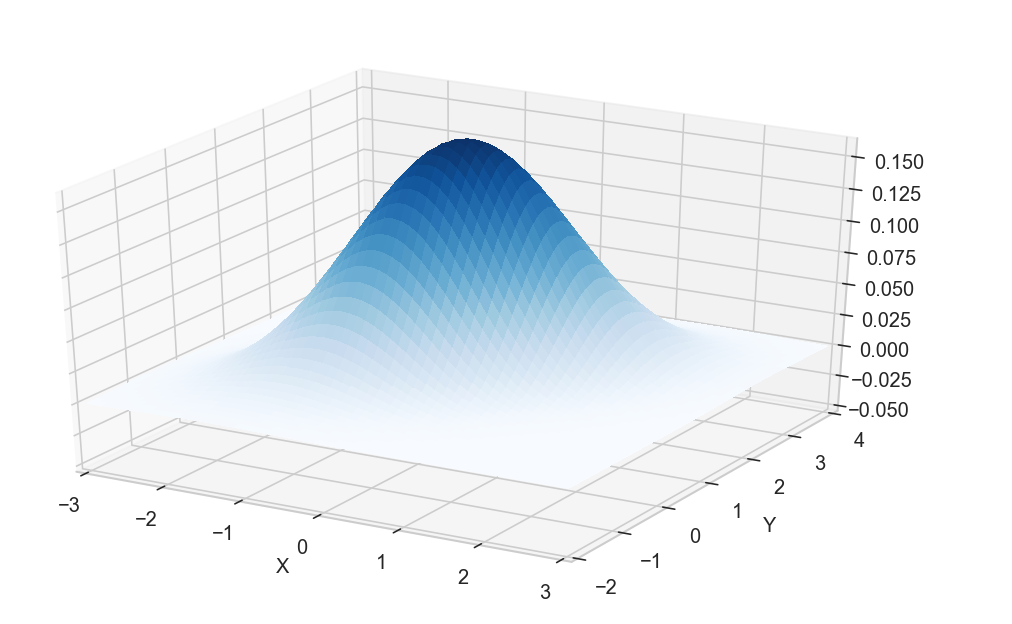
\includegraphics[scale=0.25]{two_normal_1.png}
\end{center}

Плотность двумерного нормального распределения --- это одеяло, зависшее в воздухе. При этом, под этим одеялом, по свойствам плотности распределения,  содержится объём равный единице. Если ваш объём меньше единицы, то вы можете залезть под одеяло. 

Случайные величины $X$ и $Y$ зависимы, $\Corr(X,Y) = 0.5$. Чем большие значения принимает $X$, тем, в среднем, большие значения принимает $Y$. Из-за этого их совместная плотность будет вытянута вдоль одной из осей. Если взглянуть на одеяло сверху, можно заметить это. 


\begin{center}
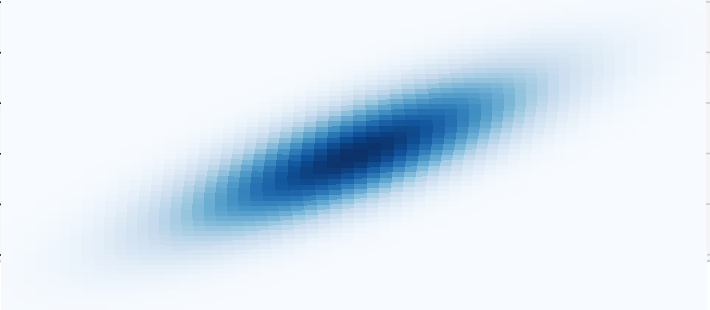
\includegraphics[scale=0.25]{two_normal_2.png}
\end{center}

От этой зависимости можно избавиться, и найти маргинальную плотность для $X$. Воспользуемся для этого формулой полной вероятности: 

\begin{multline*}
f_X(x) = \int_{-\infty}^{+\infty} f_{XY}(x,y) \dx{y} = \\ = \int_{-\infty}^{+\infty} \frac{1}{4 \pi \sqrt{0.75}} \cdot e^{-\frac{1}{2 \cdot 0.75} \cdot \left[ x^2 - x \cdot \frac{y - 1}{2} + \left( \frac{y - 1}{2}    \right)^2   \right]} \dx{y}  = \\ = \frac{1}{\sqrt{2 \pi} }\cdot e^{-\frac{x^2}{2}}.
\end{multline*}

Когда мы выинтегрировали из совместной плотности $y$, мы получили $N(0, 2^2)$. Вполне ожидаемый результат.  Если зафиксировать случайную величину $Y$ и сделать по зафиксированному значению срез, можно получить условную плотность для случайной величины $X$.  Внешний вид, а также характеристики новой плотности  будут зависеть от того, где именно мы произвели срез. Если мы это сделали в районе пика, $X \mid Y=0$,  новоиспечённая случайная величина будет обладать нулевым математическим ожиданием. По мере отдаления среза от пика математическое ожидание будет сдвигаться. 

\begin{center}
	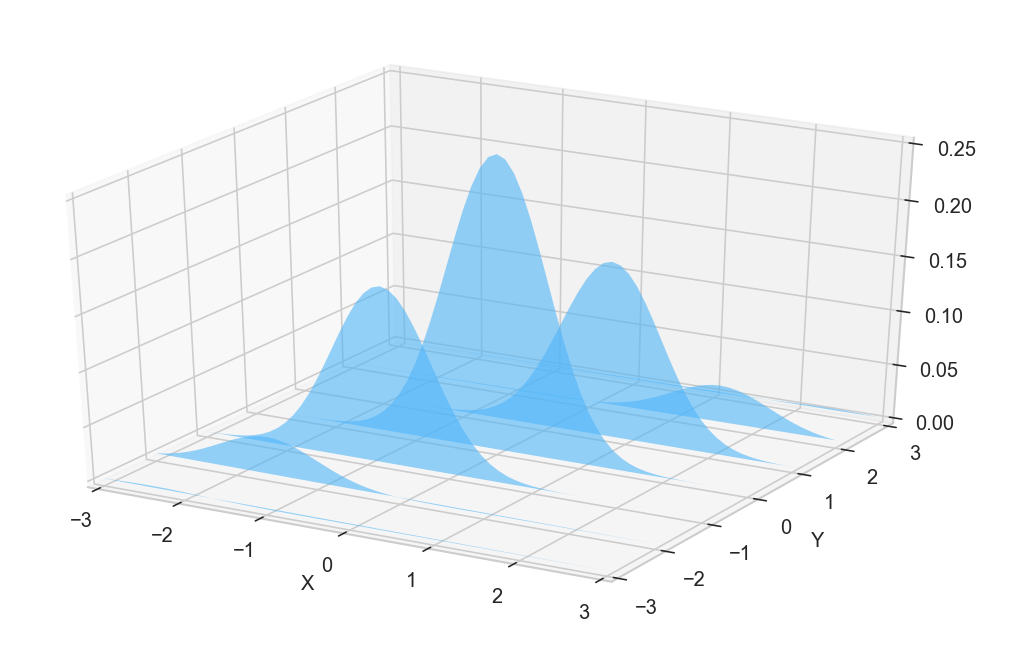
\includegraphics[scale=0.22]{two_normal_3.png}
\end{center}

В формуле условной плотности можно увидеть, как именно характеристики условного распределения зависят от точки среза

\[
f_X(x \mid Y = y)  = \frac{f(x,y)}{f_Y(y)} = \frac{1}{\sqrt{2 \cdot 0.75 \cdot \pi}} e^{-\frac{1}{2 \cdot 0.75} \cdot(x - 0.25 \cdot(y-1))^2}
\]

Если посчитать условную плотность для общего случая, можно получить, что 

\[ X \mid Y=y \sim N \left(\mu_X + \rho+{XY} \cdot \frac{\sigma_X}{\sigma_Y} \cdot(y - \mu_Y), \quad \sigma_X \cdot \sqrt{1- \rho_{XY}^2} \right).\]

В этой формуле видно, как математическое ожидание зависит от точки среза. Дисперсия зависит только от корреляции. То есть при всех срезах она одинаковая. На картинке выше это не наблюдается, так как мы произвели срез, но не сделали нормировку площади под ними к единице. После неё плотности, в плане разброса, будут выглядеть абсолютно одинаково. 


\begin{problem}{(Азартный Жора)}
Жорик взял случайную величину $X$  с плотностью распределения 

\[ 
f_X(x) = \begin{cases} 2x,  0 \le x \le 1 \\ 0, \text{ иначе} \end{cases}
\]	 

и как следует подкинул её. Выпавшее число  $x$ Виталик использовал для генерации равномерной случайной величины $Y \sim U[-x, x]$. Найдите: $f_{Y \mid X} (y)$,   $f_{XY}(x,y)$,  $f_Y(y)$,  $f_{X \mid Y} (x)$.
\end{problem}

\begin{sol}

\indef{Делай раз!} Распределение случайной величины $Y$, при условии, что $X$ приняла значение $x$ будет равномерным.  Плотность будет зависеть от того какое именно значение приняла случайная величина $X$: 

\[f_{Y \mid X}(y) = \frac{1}{2x}.\]

\indef{Делай два!} Воспользуемся формулой условной вероятности и найдём совместное 	распределение случайных величин

\[f_{XY} (x,y) = f_X(x) \cdot f_{Y \mid X} (y) =  \begin{cases} 2x \cdot \frac{1}{2x} = 1, \text{ если} 0 \le x \le 1 \text{ и } -x \le y \le x  \\ 0, \quad \text{иначе}. \end{cases} \]

\indef{Делай  три!} Из совместной плотности распределения можно найти $f_Y(y)$, выинтегрировав из неё $X$. Чтобы грамотно сделать это, нужно разобраться в структуре двумерной случайной величины. 

\begin{center}
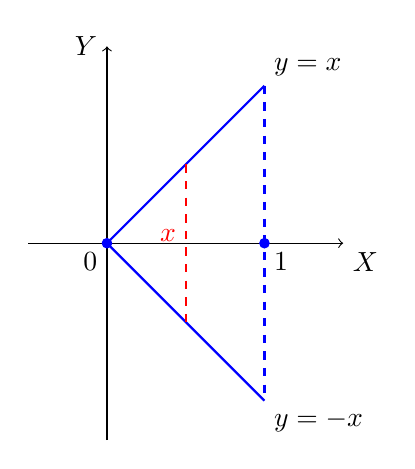
\begin{tikzpicture}
% оси
\draw [->] (-1,0) -- (3,0);
\draw [->] (0,-2.5) -- (0,2.5);	
\node [below right] at (3,0) {$X$};
\node [left] at (0,2.5) {$Y$};

% область определения функции
\node [below right] at (2,-2) {$y=-x$};
\draw [blue, thick, domain=0:2] plot (\x, {-\x});	
\node [above right] at (2,2) {$y=x$};
\draw [blue, thick, domain=0:2] plot (\x, {\x});	
\draw [blue, thick,dashed] (2,2)--(2,-2);

% точки
\draw[fill,blue] (0,0) circle [radius=0.06];
\node [below left] at (0,0) {$0$};
\draw[fill,blue] (2,0) circle [radius=0.06];
\node [below right] at (2,0) {$1$};

% икс красное
\draw [red, thick,dashed] (1,1)--(1,-1);
\node [left, red] at (1,0.1) {$x$};
\end{tikzpicture}
\end{center} 

Все свои значения случайная величина принимает внутри треугольника. За его пределами она зануляется. Обратите внимание на красную пунктирную линию. Когда виталик подкинул $X$ и она зафиксировалась, $Y$ будет варьироваться только в пределах этой красной линии. Чтобы выинтыгрировать $X$ из совместной плотности, мы должны пройтись по всем подобным красным линиям и очистить от них случайную величину $Y$.  Интеграл будет разбиваться на два кусочка. В первом случае $y > 0$ и $x$ бегает от $x = y$ до $1$. Во втором случае $ y < 0$ и $x$ бегает от $x = -y$ до $1$. 

\[ f_Y(y) = \begin{cases}\int_{-y}^1 1 \dx{x} = 1 + y, -1 \le y \le 0 \\ \int_{y}^1 1 \dx{x} = 1 - y, 0 \le y \le1 \\ 0, \text{ иначе} \end{cases} \] 

Любители модуля могут переписать первые две строчки как $1 - |y|$. При этом $x$ будет изменяться в диапазоне $|y| \le x \le  1$.  

\indef{Делай четыре!} По формуле Байеса найдём оставшуюся условную плотность. 

\[ f_{X \mid Y}(x) = \frac{f_{Y\mid X}(y) \cdot f_X(x)}{f_Y(y)} = \frac{\frac{1}{2x} \cdot 2x}{1 - |y|} = \frac{1}{1 - |y|} \]

Величину $y$ мы при этом можем выбирать на отрезке от $-1$ до $1$, а $x$ будет изменятся от $|y|$ до $1$. Попробуем на картинке понять почему так будет происходить.

\begin{center}
	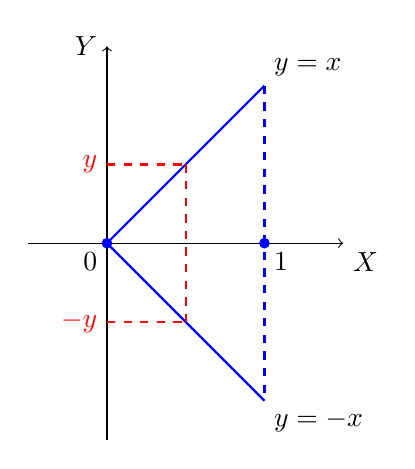
\begin{tikzpicture}
	% оси
	\draw [->] (-1,0) -- (3,0);
	\draw [->] (0,-2.5) -- (0,2.5);	
	\node [below right] at (3,0) {$X$};
	\node [left] at (0,2.5) {$Y$};
	
	% область определения функции
	\node [below right] at (2,-2) {$y=-x$};
	\draw [blue, thick, domain=0:2] plot (\x, {-\x});	
	\node [above right] at (2,2) {$y=x$};
	\draw [blue, thick, domain=0:2] plot (\x, {\x});	
	\draw [blue, thick,dashed] (2,2)--(2,-2);
	
	% точки
	\draw[fill,blue] (0,0) circle [radius=0.06];
	\node [below left] at (0,0) {$0$};
	\draw[fill,blue] (2,0) circle [radius=0.06];
	\node [below right] at (2,0) {$1$};
	
	% игрек красное
	\draw [red, thick,dashed] (1,1)--(1,-1);
	\draw [red, thick,dashed] (0,1)--(1,1);
	\draw [red, thick,dashed] (0,-1)--(1,-1);
	\node [left, red] at (0,1) {$y$};
	\node [left, red] at (0,-1) {$-y$};
	\end{tikzpicture}
\end{center} 

Когда мы фиксируем $y$, у нас появляется красная пунктирная линия, которая срезает для случайной величины $X$ все значения, находящиеся левее неё. При этом всё, что справа, случайная величина по-прежнему может принимать, и значение $y$ в знаменателе плотности распределения регулирует то, как именно при фиксации будет происходит перераспределение вероятностной массы в условной плотности.
\end{sol}


\section{Снова о формуле Байеса}

Наше погружение в чертоги разума почти окончено. Осталось вытащить наружу последние два волшебных словечка и ещё пару раз переписать формулу Байеса.  Первое слово --- \indef{априорный}. Априорными называются знания, которыми мы располагаем до эксперимента. Второе слово --- \indef{апостериорный}. Апостериорными называются знания, которыми мы обладаем после эксперимента. Новая информация уточняет наши априорные представления и трансформирует их в апостериорные с помощью формулы Байеса.

Теорема Байеса --- это основной, центральный инструмент современной статистики, на котором держится огромное число рассуждений. Чтобы увидеть это, давайте напишем формулу Байеса в том виде, в котором будем использовать по ходу книги: 

\[ 
f(\b \mid y_1, \ldots, y_n) = \frac{f(\b) \cdot f(y_1, \ldots, y_n \mid \b)}{f(y_1, \ldots, y_n)}.
\]

Здесь $y_1, \ldots, y_n$ --- это данные, которые нам удалось собрать, $\b$ --- это параметры модели, которые мы хотим оценить.   

Плотность $f(\b)$ отражает наши априорные знания о параметре $\b$ (prior).  Она является математической формализацией нашей интуиции и всех тех вещей, которые мы знали о $\b$ до проведения эксперимента. 

Плотность $f(\b \mid y_1, \ldots, y_n) $ --- это то, что мы в итоге хотим найти, распределение вероятностей параметров модели после того, как мы приняли во внимание данные, апостериорная плотность распределения (posterior).  

Функция $f(y_1, \ldots, y_n \mid \b )$ называется правдоподобием (likelihood). Из курса матстата вы должны помнить, что это вероятность появления наших данных, при условии, что все параметры модели нам известны. Мы не будем здесь вдаваться в подробности метода максимального правдоподобия. В конце главы есть несколько задачек, которые помогут читателю освежить знания. 
 
Плотность $f(y_1, \ldots, y_n)$ --- это вероятность данных, усреднённая по всем гипотезам (evidence).  Для того, чтобы найти её, часто приходится брать интегралы. Это самая страшная часть формулы Байеса. 

В концептуальном виде теорему Байеса можно переписать следующим образом

\[ 
posterior = \frac{prior \cdot likelihood}{evidence}.
\]

Давайте ещё раз вспомним пресловутую задачу про шары и коробки.  Перед нами стоит две коробки. В каждой по пять шаров. В одной из них три красных, в другой два. Мы не знаем в какой из них сколько. Наше незнание можно описать с помощью априорных вероятностей, сказав, что с вероятностью $0.5$ в правой коробке два красных шара, и с вероятностью $0.5$ три.  Как только мы засунули руку в правую коробку и вытянули из неё красный шар, мы получили наблюдение $y_1$. Для него мы можем выписать правдоподобие. 

После поступления дополнительной информации, мы пересчитываем вероятности начальных гипотез. В самом первом чуде, пересчитывая их, мы стригли деревья. Из-за этой стрижки, для того, чтобы в сумме вероятности по-прежнему давали единицу, нам нужно было делить их на полную вероятность события, то есть как раз на evidence. К счастью, самая сложная часть формулы представляет из себя нормировочную константу, и в ходе расчётов её очень часто можно игнорировать. Ничего не мешает нам вспомнить про нормировку только в самый последний момент.

\indef{Формула Байеса конвертирует информацию, которую мы пронаблюдали и наше априорное представление о природном явлении в апостериорные представления.}

\end{document}

